% Performance matrix for QEDRank formalize run 2026-10-12-e631e6a
% Generated by paper/make-tex-formalize.cjs from the run's item and reference records on 2026-10-13.
% Rebuild after a re-grade:  node paper/make-tex-formalize.cjs runs/<run-id> paper/performance-matrix-formalize.tex
%
% Each table and figure below is self-contained: copy the environments you need into the paper and
% add these packages and colours to its preamble.
\documentclass[11pt]{article}
\usepackage[a4paper,margin=2.2cm]{geometry}
\usepackage[T1]{fontenc}
\usepackage{lmodern}
\usepackage{booktabs}
\usepackage{tabularx}
\usepackage{array}
\usepackage{threeparttable}
\usepackage[font=small,labelfont=bf]{caption}
\usepackage{xcolor}
\usepackage{pgfplots}
\pgfplotsset{compat=1.18}
\definecolor{qrTimeout}{RGB}{110,110,110}
\definecolor{qrRate}{RGB}{165,165,165}
\definecolor{qrQuota}{RGB}{215,215,215}
\definecolor{qrAbst}{RGB}{86,180,233}
\definecolor{qrEnv}{RGB}{230,159,0}
\definecolor{qrImp}{RGB}{240,228,66}
\definecolor{qrScreen}{RGB}{153,153,51}
\definecolor{qrCut}{RGB}{140,81,10}
\definecolor{qrErr}{RGB}{213,94,0}
\definecolor{qrDecl}{RGB}{128,205,193}
\definecolor{qrStmt}{RGB}{204,121,167}
\definecolor{qrSorry}{RGB}{0,114,178}
\definecolor{qrAx}{RGB}{100,50,120}
\definecolor{qrOk}{RGB}{0,158,115}
\newcommand{\swatch}[1]{\textcolor{#1}{\rule{0.75em}{0.75em}}}

\begin{document}

\section*{Pilot evaluation, formalize task: performance matrix}
Run \texttt{2026-10-12-e631e6a}: 28 ProofBench papers, 84 targets per model, task \emph{formalize and prove from the paper}, 2 models.

% ---------------------------------------------------------------- Table: setup
\begin{table}[!htbp]
\centering
\caption{Evaluation setup of run \texttt{2026-10-12-e631e6a}.}
\label{tab:f-setup}
\small
\begin{tabularx}{\linewidth}{@{}>{\raggedright\arraybackslash}p{2.4cm}>{\raggedright\arraybackslash}X@{}}
\toprule
Corpus & \texttt{ProofBench} at commit \texttt{e631e6a} (2026-10-10), folder \texttt{ProofBench/PROBLEMS}: 29 paper folders, of which 28 with a PDF were run (P054 has no PDF). Three targets per paper (main theorem, upper bound, lower bound): 84 targets per model. Claim status from the benchmark index: main theorems 27 established, 1 uncertain; bounds 56 uncertain. Difficulty label: Research 27, unlabelled 1. \\
Task & Formalize and prove from the paper. The prompt names the target and gives up to 24{,}000 characters of passages extracted from the paper's PDF.\textsuperscript{b} The model returns (A) a Lean statement of the claim with any definitions it needs, (B) a complete Lean proof file, or no file if it cannot prove the claim, (C) a paper-to-Lean mapping, and (D) two confidences from 0 to 100: that A is faithful and that B passes the audit. \\
Protocol & One request per target (pass@1), no repair rounds, no tools or retrieval; prompt template \texttt{qedrank-prompt-v2}. \\
Models & \textbf{Kimi K3}: \texttt{kimi-k3} via \texttt{api.moonshot.ai}; 2.8\,T parameters, 104\,B active (mixture of experts); released 2026-07-16; temperature 0.\newline \textbf{Qwen3-30B-A3B}: \texttt{qwen3-30b-a3b-instruct-2507} via \texttt{chat-ai.academiccloud.de}; 30.5\,B parameters, 3.3\,B active (mixture of experts); released 2025-07-30; temperature 0. \\
Budgets & 16{,}384 output tokens and 300\,s per request. \\
Grader & Lean v4.34.1, Mathlib \texttt{d13f23b} (the toolchain named in the prompt); 400{,}000 heartbeats, 600\,s and 8\,GB per compilation.\textsuperscript{a} Part A is compiled on its own; it is \emph{faithful} when it compiles and is accepted as equivalent to the audited reference statement (definitional identity, an automated two-way implication, or expert review). Part B is \emph{verified} when it compiles, contains the target theorem, that theorem's statement is an accepted match, it depends only on \texttt{propext}, \texttt{Classical.choice} and \texttt{Quot.sound}, and the claim is established. \\
Harness & QEDRank commit \texttt{bfc8df88f2}; total wall-clock time 2.5\,h. \\
Statistics & Exact two-sided 95\,\% Clopper--Pearson intervals over targets. The three targets of a paper are not independent, so pooled intervals are too narrow; the primary endpoint has one target per paper. \\
\bottomrule
\end{tabularx}
\par\smallskip\parbox{\linewidth}{\footnotesize \textsuperscript{a}\,Graded in the QEDRank default Lean project (\texttt{lean}). The benchmark pins Lean v4.33.1, Mathlib v4.33.1, the Matroid library at \texttt{fa6c155} and the option \texttt{maxSynthPendingDepth = 3}; its reference files import benchmark modules that this project does not contain (Table~\ref{tab:f-refs}). \textsuperscript{b}\,None of the 168 prompts contained definitions from the benchmark's Lean files, so the model had to define every notion itself.}
\end{table}

% ---------------------------------------------------------------- Table: reference availability
\begin{table}[!htbp]
\centering
\begin{threeparttable}
\caption{Reference statements available to the grader, by target. A model statement can only be checked for faithfulness against an available reference.}
\label{tab:f-refs}
\small
\setlength{\tabcolsep}{4.5pt}
\begin{tabular}{@{}lrrrrrrrr@{}}
\toprule
 & & & \multicolumn{2}{c}{Unavailable because} & \multicolumn{3}{c}{Reference proof} & \\
\cmidrule(lr){4-5}\cmidrule(lr){6-8}
Target & Targets & Available & Library\tnote{a} & Wrapper\tnote{b} & Complete & \texttt{sorry} & Not compiled & Established \\
\midrule
Main theorem & 28 & 16 & 9 & 3 & 0 & 19 & 9 & 27 \\
Upper bound & 28 & 0 & 28 & 0 & 0 & 0 & 28 & 0 \\
Lower bound & 28 & 0 & 28 & 0 & 0 & 0 & 28 & 0 \\
\midrule
All & 84 & 16 & 65 & 3 & 0 & 19 & 65 & 27 \\
\bottomrule
\end{tabular}
\begin{tablenotes}\footnotesize
\item[a] The reference file imports modules that are not in the grader's Lean project (\texttt{ProofBench.PROBLEMS} 62, \texttt{ProofBench.Mathlib} 11, \texttt{ProofBench.Mathlib\_Problems} 4, \texttt{Matroid} 2, \texttt{Archive} 1 imports), so its statement could not be compiled. This is a property of the grader configuration, not of the benchmark.
\item[b] The statement compiled in the benchmark's own file but failed after QEDRank wrapped it in its comparison namespace (\textit{unexpected name after \texttt{end}}); a defect of the harness.
\item[] \textit{Reference proof}: \emph{complete} has no \texttt{sorry}; \emph{\texttt{sorry}} compiles with a placeholder; \emph{not compiled} could not be compiled in the grader's project. \emph{Established}: the claim is marked established in the benchmark index (all bounds are marked uncertain).
\end{tablenotes}
\end{threeparttable}
\end{table}

% ---------------------------------------------------------------- Table: outcome breakdown
\begin{table}[!htbp]
\centering
\caption{Outcome of every request, by model (84 targets each). Within each part the categories are mutually exclusive; each target is assigned to the first step at which it stopped.}
\label{tab:f-outcomes}
\small
\begin{tabular}{@{}lrr@{}}
\toprule
Outcome & Kimi K3 & Qwen3-30B-A3B \\
\midrule
\addlinespace[2pt]\multicolumn{3}{@{}l}{\textbf{Part A: statement} (each target counted once)} \\
\addlinespace[1pt]\multicolumn{3}{@{}l}{\quad\textit{Provider (not attributable to the model)}} \\
\qquad\swatch{qrTimeout}\,Request timed out & 0 (0.0\,\%) & 7 (8.3\,\%) \\
\qquad\swatch{qrRate}\,Refused: concurrency limit (HTTP 429) & 14 (16.7\,\%) & 0 (0.0\,\%) \\
\qquad\swatch{qrQuota}\,Refused: account balance exhausted (HTTP 429) & 70 (83.3\,\%) & 0 (0.0\,\%) \\
\addlinespace[1pt]\multicolumn{3}{@{}l}{\quad\textit{Model}} \\
\qquad\swatch{qrCut}\,No statement: answer cut off at the token limit & 0 (0.0\,\%) & 31 (36.9\,\%) \\
\qquad\swatch{qrAbst}\,No statement: part A not in a Lean code block & 0 (0.0\,\%) & 2 (2.4\,\%) \\
\qquad\swatch{qrImp}\,Statement imports a module that does not exist & 0 (0.0\,\%) & 3 (3.6\,\%) \\
\qquad\swatch{qrErr}\,Statement does not compile & 0 (0.0\,\%) & 41 (48.8\,\%) \,{\footnotesize(4 cut off)} \\
\midrule
\addlinespace[2pt]\multicolumn{3}{@{}l}{\textbf{Part B: proof file} (answered targets only)} \\
\qquad\swatch{qrAbst}\,No proof file returned & --- & 2 (2.6\,\%) \\
\qquad\swatch{qrCut}\,No proof file extracted (answer cut off) & --- & 32 (41.6\,\%) \\
\qquad\swatch{qrDecl}\,Proof declined: file contains only comments & --- & 12 (15.6\,\%) \\
\qquad\swatch{qrErr}\,Does not compile & --- & 31 (40.3\,\%) \\
\midrule
Targets & 84 & 84 \\
\bottomrule
\end{tabular}
\par\smallskip\parbox{0.94\linewidth}{\footnotesize \textit{Cut off}: the answer reached the 16{,}384-token output limit before it ended. \textit{Imports a module that does not exist}: Lean reports a missing object file, and no package of the grader's Lean project has a source file for that module; the grader itself labels these items infrastructure failures. \textit{Proof declined}: the proof file has no Lean code, only comments saying that no complete proof is given, which the prompt allows; the grader itself counts these files as compiled.}
\end{table}

% ---------------------------------------------------------------- Figure: outcome composition
\begin{figure}[!htbp]
\centering
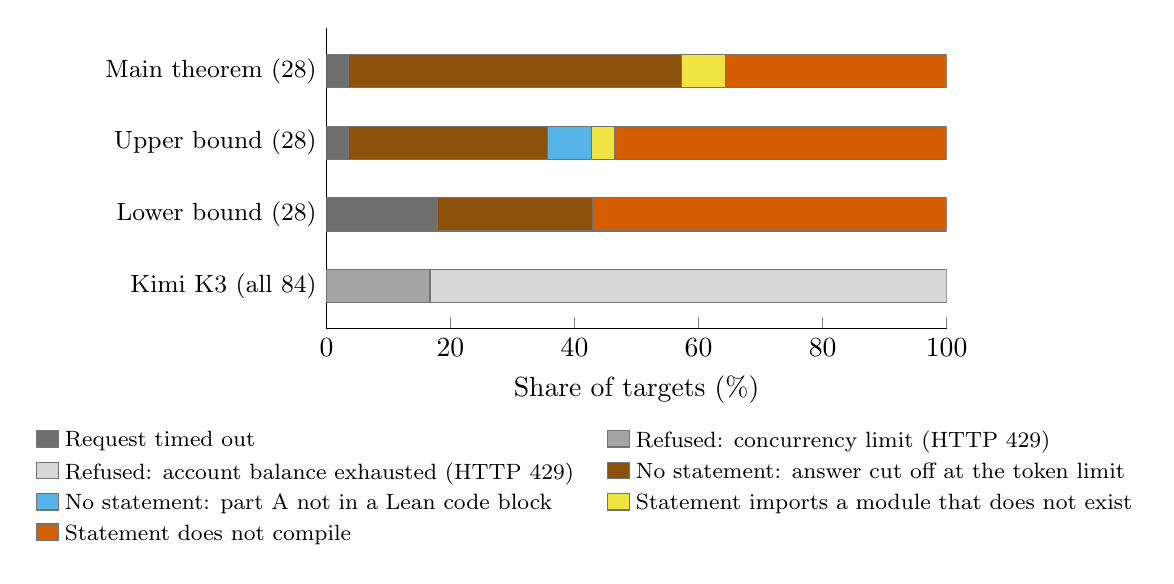
\begin{tikzpicture}
\begin{axis}[
  xbar stacked, bar width=12pt, width=0.78\linewidth, height=5.4cm,
  xmin=0, xmax=100, xlabel={Share of targets (\%)},
  ytick={0,1,2,3}, yticklabels={{Kimi K3 (all 84)},{Lower bound (28)},{Upper bound (28)},{Main theorem (28)}},
  ymin=-0.6, ymax=3.6, y tick label style={font=\small},
  legend style={at={(0.42,-0.30)}, anchor=north, legend columns=2, draw=none, font=\footnotesize,
    /tikz/every even column/.append style={column sep=10pt}},
  legend cell align=left, axis x line*=bottom, axis y line*=left,
]
\addplot[fill=qrTimeout, draw=black!55] coordinates {(0.0,0) (17.9,1) (3.6,2) (3.6,3)};
\addplot[fill=qrRate, draw=black!55] coordinates {(16.7,0) (0.0,1) (0.0,2) (0.0,3)};
\addplot[fill=qrQuota, draw=black!55] coordinates {(83.3,0) (0.0,1) (0.0,2) (0.0,3)};
\addplot[fill=qrCut, draw=black!55] coordinates {(0.0,0) (25.0,1) (32.1,2) (53.6,3)};
\addplot[fill=qrAbst, draw=black!55] coordinates {(0.0,0) (0.0,1) (7.1,2) (0.0,3)};
\addplot[fill=qrImp, draw=black!55] coordinates {(0.0,0) (0.0,1) (3.6,2) (7.1,3)};
\addplot[fill=qrErr, draw=black!55] coordinates {(0.0,0) (57.1,1) (53.6,2) (35.7,3)};
\legend{{Request timed out},{Refused: concurrency limit (HTTP 429)},{Refused: account balance exhausted (HTTP 429)},{No statement: answer cut off at the token limit},{No statement: part A not in a Lean code block},{Statement imports a module that does not exist},{Statement does not compile}}
\end{axis}
\end{tikzpicture}
\caption{Where part A ended, as a share of each group's targets (Qwen3-30B-A3B by target; Kimi K3 over all targets). Grey: provider failures; the other colours are outcomes attributable to the model (Table~\ref{tab:f-outcomes}).}
\label{fig:f-outcomes}
\end{figure}

% ---------------------------------------------------------------- Table: performance matrix
\begin{table}[!htbp]
\centering
\begin{threeparttable}
\caption{Performance matrix (task: formalize and prove from the paper, pass@1). Rates exclude provider failures and items the grader could not evaluate.}
\label{tab:f-matrix}
\small
\begin{tabular}{@{}lrr@{}}
\toprule
Measure & Kimi K3 & Qwen3-30B-A3B \\
\midrule
Targets run (28 papers $\times$ 3) & 84 & 84 \\
Requests timed out & 0 & 7 \\
Refused: concurrency limit (HTTP 429) & 14 & 0 \\
Refused: account balance exhausted & 70 & 0 \\
Answered & 0 & 77 \\
Answer cut off at the token limit & --- & 35/77 (45.5\,\%) \\
\quad of which repetition loops\tnote{a} & --- & 30/35 \\
\midrule
\multicolumn{3}{@{}l}{\textit{Part A: statement}} \\
Statement extracted from the answer & --- & 44/77 (57.1\,\%) \\
Statement compiles\tnote{b} & --- & 0/77 (0.0\,\%) \\
\quad 95\,\% CI & --- & [0.0, 4.7] \\
Reference statement available\tnote{c} & 16/84 & 16/84 \\
Statement faithful to the reference\tnote{d} & --- & 0/15 (0.0\,\%) \\
\quad 95\,\% CI & --- & [0.0, 21.8] \\
\midrule
\multicolumn{3}{@{}l}{\textit{Part B: proof}} \\
Proof declined in comments\tnote{e} & --- & 12/77 (15.6\,\%) \\
Proof file with Lean code & --- & 31/77 (40.3\,\%) \\
Proof file compiles (of files with code) & --- & 0/31 (0.0\,\%) \\
\textbf{Verified pass@1, main theorem}\tnote{f} & --- & \textbf{0/15 (0.0\,\%)} \\
\quad 95\,\% CI & --- & [0.0, 21.8] \\
\midrule
Compile rate as reported by QEDRank\tnote{g} & --- & 10/72 (13.9\,\%) \\
\midrule
Mean stated confidence: statement faithful\tnote{h} & --- & 97\,\% {\footnotesize(n\,=\,42)} \\
Mean stated confidence: proof passes audit\tnote{h} & --- & 13\,\% {\footnotesize(n\,=\,42)} \\
Median latency per answer & --- & 87.2\,s \\
Median output tokens per answer & --- & 4{,}109 \\
\bottomrule
\end{tabular}
\begin{tablenotes}\footnotesize
\item[a] At least 90\,\% of the answer's non-empty lines repeat an earlier line (Figure~\ref{fig:f-length}).
\item[b] Answered targets whose part A file compiles on its own. Answers without an extractable statement count as failures.
\item[c] Targets whose audited reference statement compiled in the grader's project (Table~\ref{tab:f-refs}); only these can be checked for faithfulness.
\item[d] Denominator: targets with an available reference, excluding provider failures. A statement that does not compile counts as not faithful.
\item[e] The proof file holds only comments stating that no complete proof is given, as the prompt allows when the model cannot prove the claim.
\item[f] Primary endpoint. Denominator: main theorems with an available reference and an established claim, excluding provider failures.
\item[g] QEDRank's own summary figure: part B files that compiled, among answers with a proof file. It counts the comment-only files of note e as compiled; reported for comparison only.
\item[h] The model's own estimates in part D, averaged over answers that stated one.
\item[] Kimi K3: no request was answered (Table~\ref{tab:f-outcomes}), so no rate is defined and no comparison between the models is made.
\end{tablenotes}
\end{threeparttable}
\end{table}

% ---------------------------------------------------------------- Figure: attrition
\begin{figure}[!htbp]
\centering
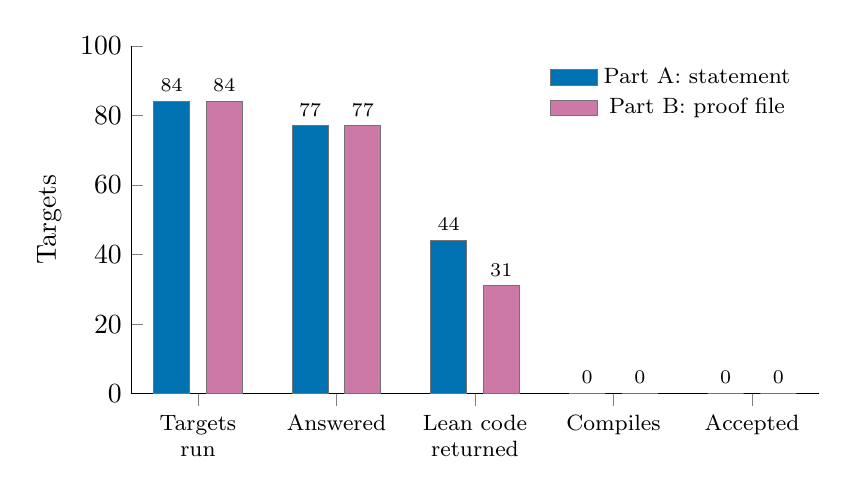
\begin{tikzpicture}
\begin{axis}[
  ybar=6pt, bar width=13pt, width=0.85\linewidth, height=6cm, area legend,
  ymin=0, ymax=100, ylabel={Targets},
  xtick={1,...,5}, xticklabels={{Targets\\run},{Answered},{Lean code\\returned},{Compiles},{Accepted}},
  xticklabel style={align=center, font=\footnotesize}, enlarge x limits=0.12,
  nodes near coords, every node near coord/.append style={font=\scriptsize},
  legend style={at={(0.98,0.97)}, anchor=north east, draw=none, font=\footnotesize},
  axis x line*=bottom, axis y line*=left,
]
\addplot[fill=qrSorry, draw=black!55] coordinates {(1,84) (2,77) (3,44) (4,0) (5,0)};
\addplot[fill=qrStmt, draw=black!55] coordinates {(1,84) (2,77) (3,31) (4,0) (5,0)};
\legend{Part A: statement, Part B: proof file}
\end{axis}
\end{tikzpicture}
\caption{Attrition from request to accepted result for Qwen3-30B-A3B. \emph{Lean code returned}: a statement could be extracted (part A) or the proof file contains Lean code (part B). \emph{Accepted}: faithful to the reference (part A, 15 eligible targets) or verified (part B, 15 eligible main theorems).}
\label{fig:f-attrition}
\end{figure}

% ---------------------------------------------------------------- Table: by target
\begin{table}[!htbp]
\centering
\caption{Results by target (Qwen3-30B-A3B).}
\label{tab:f-targets}
\small
\begin{tabular}{@{}lrrrr@{}}
\toprule
Measure & Main theorem & Upper bound & Lower bound & All \\
\midrule
Targets run & 28 & 28 & 28 & 84 \\
Requests failed at the provider & 1 & 1 & 5 & 7 \\
Answered & 27 & 27 & 23 & 77 \\
Answer cut off at the token limit & 15 & 12 & 8 & 35 \\
Statement extracted & 12 & 16 & 16 & 44 \\
Statement compiles & 0 & 0 & 0 & 0 \\
Reference statement available & 16 & 0 & 0 & 16 \\
Statement faithful & 0/15 & --- & --- & 0/15 \\
Proof declined in comments & 4 & 3 & 5 & 12 \\
Proof file with Lean code & 8 & 12 & 11 & 31 \\
Proof file compiles & 0 & 0 & 0 & 0 \\
Verified (main theorem, eligible) & 0/15 & --- & --- & 0/15 \\
\bottomrule
\end{tabular}
\end{table}

% ---------------------------------------------------------------- Table: per-paper grid
\begin{table}[!htbp]
\centering
\caption{Part A outcome for every paper and target (Qwen3-30B-A3B). Kimi K3 answered no request and is omitted.}
\label{tab:f-grid}
\footnotesize
\renewcommand{\arraystretch}{0.92}
\begin{tabular}{@{}llllll@{}}
\toprule

Paper & Main claim & Ref. & Main & Upper & Lower \\
\midrule
P014 & established & --\,--\,-- & \swatch{qrCut}\,\texttt{CUT} & \swatch{qrErr}\,\texttt{ERR}\textsuperscript{d} & \swatch{qrCut}\,\texttt{CUT} \\
P015 & established & --\,--\,-- & \swatch{qrErr}\,\texttt{ERR} & \swatch{qrErr}\,\texttt{ERR} & \swatch{qrErr}\,\texttt{ERR} \\
P026 & established & M\,--\,-- & \swatch{qrErr}\,\texttt{ERR}\textsuperscript{d} & \swatch{qrErr}\,\texttt{ERR} & \swatch{qrErr}\,\texttt{ERR}\textsuperscript{d} \\
P037 & established & --\,--\,-- & \swatch{qrImp}\,\texttt{IMP}\textsuperscript{d} & \swatch{qrErr}\,\texttt{ERR}\textsuperscript{d} & \swatch{qrErr}\,\texttt{ERR}\textsuperscript{d} \\
P047 & established & M\,--\,-- & \swatch{qrCut}\,\texttt{CUT} & \swatch{qrCut}\,\texttt{CUT} & \swatch{qrCut}\,\texttt{CUT} \\
P048 & established & M\,--\,-- & \swatch{qrCut}\,\texttt{CUT} & \swatch{qrCut}\,\texttt{CUT} & \swatch{qrCut}\,\texttt{CUT} \\
P049 & established & M\,--\,-- & \swatch{qrCut}\,\texttt{CUT} & \swatch{qrCut}\,\texttt{CUT} & \swatch{qrCut}\,\texttt{CUT} \\
P050 & established & M\,--\,-- & \swatch{qrCut}\,\texttt{CUT} & \swatch{qrCut}\,\texttt{CUT} & \swatch{qrTimeout}\,\texttt{TO} \\
P051 & uncertain & M\,--\,-- & \swatch{qrTimeout}\,\texttt{TO} & \swatch{qrCut}\,\texttt{CUT} & \swatch{qrErr}\,\texttt{ERR} \\
P052 & established & M\,--\,-- & \swatch{qrErr}\,\texttt{ERR} & \swatch{qrCut}\,\texttt{CUT} & \swatch{qrErr}\,\texttt{ERR} \\
P053 & established & M\,--\,-- & \swatch{qrCut}\,\texttt{CUT} & \swatch{qrErr}\,\texttt{ERR} & \swatch{qrCut}\,\texttt{CUT} \\
P056 & established & --\,--\,-- & \swatch{qrCut}\,\texttt{CUT} & \swatch{qrAbst}\,\texttt{FMT} & \swatch{qrErr}\,\texttt{ERR} \\
P071 & established & M\,--\,-- & \swatch{qrCut}\,\texttt{CUT} & \swatch{qrErr}\,\texttt{ERR} & \swatch{qrTimeout}\,\texttt{TO} \\
P094 & established & M\,--\,-- & \swatch{qrCut}\,\texttt{CUT} & \swatch{qrCut}\,\texttt{CUT} & \swatch{qrTimeout}\,\texttt{TO} \\
P095 & established & M\,--\,-- & \swatch{qrCut}\,\texttt{CUT} & \swatch{qrErr}\,\texttt{ERR} & \swatch{qrCut}\,\texttt{CUT} \\
P096 & established & M\,--\,-- & \swatch{qrErr}\,\texttt{ERR}\textsuperscript{d} & \swatch{qrErr}\,\texttt{ERR} & \swatch{qrErr}\,\texttt{ERR}\textsuperscript{d} \\
P097 & established & M\,--\,-- & \swatch{qrCut}\,\texttt{CUT} & \swatch{qrAbst}\,\texttt{FMT} & \swatch{qrTimeout}\,\texttt{TO} \\
P099 & established & M\,--\,-- & \swatch{qrErr}\,\texttt{ERR} & \swatch{qrErr}\,\texttt{ERR} & \swatch{qrErr}\,\texttt{ERR} \\
P100 & established & M\,--\,-- & \swatch{qrErr}\,\texttt{ERR} & \swatch{qrErr}\,\texttt{ERR} & \swatch{qrErr}\,\texttt{ERR} \\
P101 & established & M\,--\,-- & \swatch{qrErr}\,\texttt{ERR} & \swatch{qrErr}\,\texttt{ERR} & \swatch{qrErr}\,\texttt{ERR} \\
P102 & established & --\,--\,-- & \swatch{qrCut}\,\texttt{CUT} & \swatch{qrErr}\,\texttt{ERR} & \swatch{qrErr}\,\texttt{ERR} \\
P103 & established & --\,--\,-- & \swatch{qrCut}\,\texttt{CUT} & \swatch{qrCut}\,\texttt{CUT} & \swatch{qrCut}\,\texttt{CUT} \\
P104 & established & --\,--\,-- & \swatch{qrCut}\,\texttt{CUT} & \swatch{qrCut}\,\texttt{CUT} & \swatch{qrTimeout}\,\texttt{TO} \\
P105 & established & --\,--\,-- & \swatch{qrErr}\,\texttt{ERR} & \swatch{qrErr}\,\texttt{ERR} & \swatch{qrErr}\,\texttt{ERR} \\
P106 & established & --\,--\,-- & \swatch{qrCut}\,\texttt{CUT} & \swatch{qrTimeout}\,\texttt{TO} & \swatch{qrErr}\,\texttt{ERR} \\
P107 & established & --\,--\,-- & \swatch{qrImp}\,\texttt{IMP} & \swatch{qrImp}\,\texttt{IMP}\textsuperscript{d} & \swatch{qrErr}\,\texttt{ERR}\textsuperscript{d} \\
P108 & established & --\,--\,-- & \swatch{qrErr}\,\texttt{ERR}\textsuperscript{d} & \swatch{qrErr}\,\texttt{ERR} & \swatch{qrErr}\,\texttt{ERR}\textsuperscript{d} \\
P109 & established & --\,--\,-- & \swatch{qrErr}\,\texttt{ERR} & \swatch{qrErr}\,\texttt{ERR} & \swatch{qrErr}\,\texttt{ERR} \\
\bottomrule
\end{tabular}
\par\smallskip\parbox{0.92\linewidth}{\footnotesize \texttt{TO} Request timed out; \texttt{CUT} no statement, answer cut off at the token limit; \texttt{FMT} no statement, part A not in a Lean code block; \texttt{IMP} imports a module that does not exist; \texttt{ERR} does not compile. \textsuperscript{d}\,proof declined in comments. \textit{Ref.}: targets with an available reference statement (M main theorem, U upper bound, L lower bound).}
\end{table}

% ---------------------------------------------------------------- Figure: output length
\begin{figure}[!htbp]
\centering
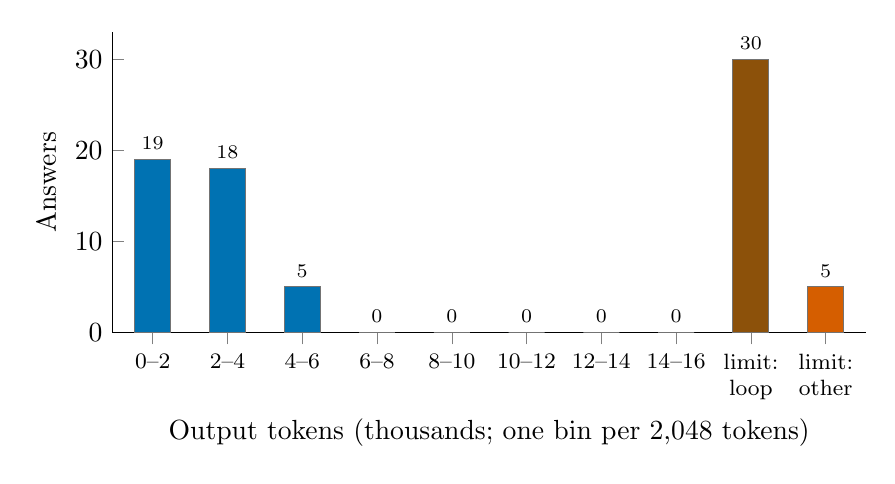
\begin{tikzpicture}
\begin{axis}[
  ybar, bar width=13pt, width=0.92\linewidth, height=5.4cm,
  ymin=0, ylabel={Answers}, xlabel={Output tokens (thousands; one bin per 2{,}048 tokens)},
  xtick={1,...,10}, xticklabels={0--2,2--4,4--6,6--8,8--10,10--12,12--14,14--16,{limit:\\loop},{limit:\\other}}, xticklabel style={font=\footnotesize, align=center},
  nodes near coords, every node near coord/.append style={font=\scriptsize},
  enlarge x limits=0.06, axis x line*=bottom, axis y line*=left,
]
\addplot[fill=qrSorry, draw=black!55, bar shift=0pt] coordinates {(1,19) (2,18) (3,5) (4,0) (5,0) (6,0) (7,0) (8,0)};
\addplot[fill=qrCut, draw=black!55, bar shift=0pt] coordinates {(9,30)};
\addplot[fill=qrErr, draw=black!55, bar shift=0pt] coordinates {(10,5)};
\end{axis}
\end{tikzpicture}
\caption{Length of the 77 answers of Qwen3-30B-A3B. 35 answers (45\,\%) reached the 16{,}384-token limit. In 30 of them at least 90\,\% of the lines repeat an earlier line (29 repeat \texttt{import} lines); the other 5 were long answers cut off before they ended.}
\label{fig:f-length}
\end{figure}

% ---------------------------------------------------------------- Figure: statement error taxonomy
\begin{figure}[!htbp]
\centering
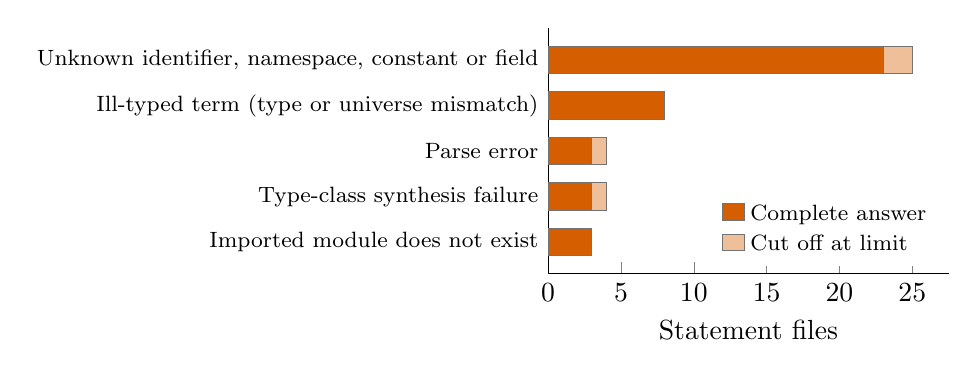
\begin{tikzpicture}
\begin{axis}[
  xbar stacked, bar width=10pt, width=0.55\linewidth, height=4.7cm,
  xmin=0, xlabel={Statement files}, ytick={0,1,2,3,4},
  yticklabels={{Imported module does not exist},{Type-class synthesis failure},{Parse error},{Ill-typed term (type or universe mismatch)},{Unknown identifier, namespace, constant or field}}, y tick label style={font=\footnotesize},
  ymin=-0.7, ymax=4.7,
  legend style={at={(0.98,0.03)}, anchor=south east, draw=none, fill=white, font=\footnotesize}, legend cell align=left,
  axis x line*=bottom, axis y line*=left,
]
\addplot[fill=qrErr, draw=black!55] coordinates {(3,0) (3,1) (3,2) (8,3) (23,4)};
\addplot[fill=qrErr!40, draw=black!55] coordinates {(0,0) (1,1) (1,2) (0,3) (2,4)};
\legend{Complete answer, Cut off at limit}
\end{axis}
\end{tikzpicture}
\caption{First Lean error of the 44 extracted statements of Qwen3-30B-A3B that did not compile. \emph{Unknown identifier} includes names the model used without importing or defining them (Lean's \texttt{autoImplicit} hint).}
\label{fig:f-errors}
\end{figure}

% ---------------------------------------------------------------- Figure: stated confidence
\begin{figure}[!htbp]
\centering
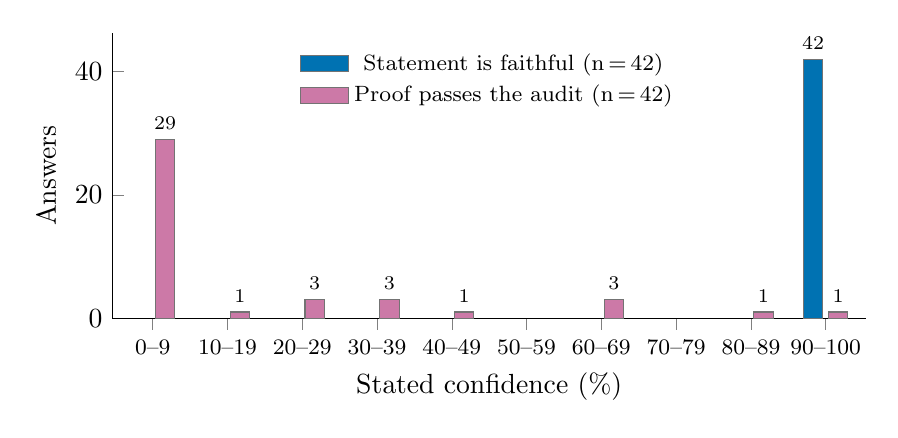
\begin{tikzpicture}
\begin{axis}[
  ybar=2pt, bar width=7pt, width=0.92\linewidth, height=5.2cm, area legend,
  ymin=0, ylabel={Answers}, xlabel={Stated confidence (\%)},
  xtick={1,...,10}, xticklabels={0--9,10--19,20--29,30--39,40--49,50--59,60--69,70--79,80--89,90--100}, xticklabel style={font=\footnotesize},
  y filter/.expression={y==0 ? nan : y}, unbounded coords=discard,
  nodes near coords, every node near coord/.append style={font=\scriptsize},
  legend style={at={(0.5,0.97)}, anchor=north, draw=none, font=\footnotesize},
  enlarge x limits=0.06, axis x line*=bottom, axis y line*=left,
]
\addplot[fill=qrSorry, draw=black!55] coordinates {(1,0) (2,0) (3,0) (4,0) (5,0) (6,0) (7,0) (8,0) (9,0) (10,42)};
\addplot[fill=qrStmt, draw=black!55] coordinates {(1,29) (2,1) (3,3) (4,3) (5,1) (6,0) (7,3) (8,0) (9,1) (10,1)};
\legend{Statement is faithful (n\,=\,42), Proof passes the audit (n\,=\,42)}
\end{axis}
\end{tikzpicture}
\caption{Confidence that Qwen3-30B-A3B stated in part D. Of the same answers, 0 statements compiled and 0 proof files with Lean code compiled.}
\label{fig:f-confidence}
\end{figure}

\clearpage
% ---------------------------------------------------------------- Observations (numbers from the tables above)
\subsection*{Observations}
\begin{itemize}\setlength\itemsep{2pt}
\item Qwen3-30B-A3B: 0 of 77 answered targets produced a statement that compiles (95\,\% CI [0.0, 4.7]\,\%). For 33 answers no statement could be extracted, 31 of them because the answer ran into the token limit.
\item The most frequent first error of a failed statement is \emph{unknown identifier, namespace, constant or field} (25 of 44): the model used Mathlib names it had not imported, names that do not exist, or notions it never defined. 3 statements import a Mathlib module that does not exist.
\item 12 answers declined the proof in comments, as the prompt allows; 0 of the 31 proof files with Lean code compiled, and no target was verified (0/15 eligible main theorems).
\item The model's stated confidence that its statement is faithful averaged 97\,\% (42 answers), while 0 of its statements compiled (Figure~\ref{fig:f-confidence}).
\end{itemize}

% ---------------------------------------------------------------- Threats to validity (adapt to the paper)
\subsection*{Threats to validity}
\begin{itemize}\setlength\itemsep{2pt}
\item \textbf{Reference statements.} The run was graded in QEDRank's default Lean project rather than the benchmark's pinned project. The model answers were compiled with the toolchain named in the prompt, but 65 of the 84 reference statements import benchmark modules that this project does not contain, and 3 more failed because of a defect in QEDRank's statement wrapper (Table~\ref{tab:f-refs}). Faithfulness can therefore be measured on 16 main theorems at most, and on no upper or lower bound.
\item \textbf{No benchmark definitions in the prompt.} No prompt contained the definitions of the benchmark's Lean files, so each model statement introduces its own notions. Even a statement that compiles would rarely be decided equivalent to the reference automatically; expert review would be needed.
\item \textbf{Grader labels corrected.} QEDRank's summary counts 10 comment-only proof files as compiled and labels 3 statements that import non-existent modules as infrastructure failures. The tables above count them as declined proofs and model errors.
\item \textbf{Provider failures.} Kimi K3 answered none of its 84 requests: 14 were refused because the account allows one concurrent request, 70 because the account was suspended for insufficient balance. No comparison between models is possible from this run.
\item \textbf{Decoding.} Qwen3-30B-A3B ran at temperature 0. 35 of 77 answers reached the token limit, 30 of them in a repetition loop. Its model card recommends temperature 0.7, top-p 0.8 and top-k 20, and a presence penalty between 0 and 2 to reduce endless repetitions; the output budget matches the 16{,}384 tokens it recommends. A rerun with the recommended sampling settings may change the extraction and compile rates.
\item \textbf{Single attempt.} One request per target, without repair rounds or tools; pass@$k$ and repair success are not measured. 27 of the 28 papers are labelled research-level and 1 unlabelled, so the run says nothing about easier problems.
\item \textbf{Contamination.} Neither provider states a training cutoff and the problems' publication dates are not recorded, so prior exposure cannot be assessed.
\end{itemize}

\end{document}
